\begin{scanpage}{0189}{171}
\begin{minipage}[t]{.43\linewidth}\vspace{0pt}\centering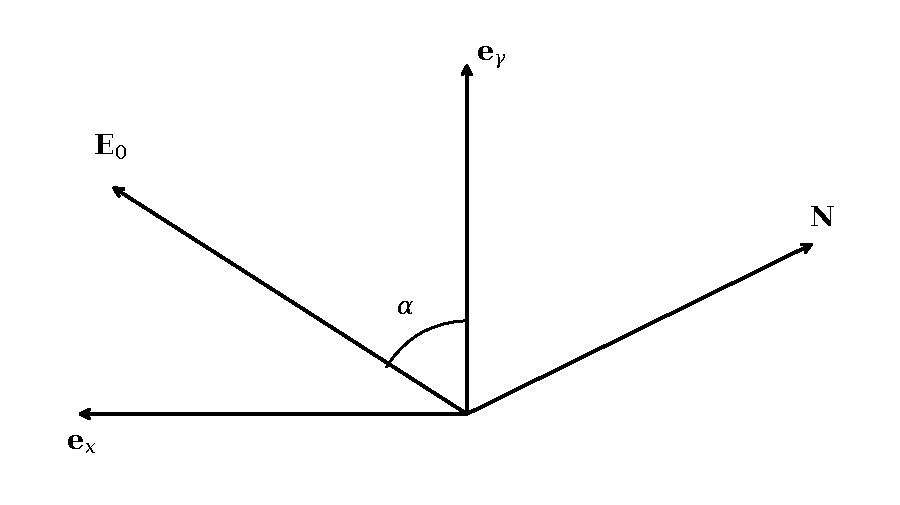
\includegraphics[width=.95\linewidth]{images/recreated/c-0189-fig72.pdf}\par Figure 72.\end{minipage}\hfill
\begin{minipage}[t]{.53\linewidth}\vspace{0pt}
source Q is in the plane yOz, and radiates a linearly polarized wave. Furthermore, we shall assume that the polarizer P which is shown in Figure 69 is now absent.

Let us designate by $\alpha$ the angle between the plane yOz and the incident wave electric vector $\mathbf E_0$ (Figure 72). The field of this wave will be represented in the form
\end{minipage}
\[
\begin{aligned}E_x=H_{0\gamma}&=E_{0x}e^{ik(y\sin\gamma+z\cos\gamma)},\\
H_x=-E_{0\gamma}&=H_{0x}e^{ik(y\sin\alpha+z\cos\gamma)},
\end{aligned}\tag{27.01}
\]
where
\[
E_{0x}=E_0\sin\alpha,\quad H_{0x}=-E_0\cos\alpha,\quad\frac{E_{0x}}{E_{0\gamma}}=\operatorname{tg}\alpha.\tag{27.02}
\]
The field scattered by the body is determined in the wave zone by the equations
\[
\left.\begin{aligned}E_\varphi=-H_\vartheta&=\frac{ia}2[E_{0x}\overline\Sigma_1(\gamma,\vartheta,\varphi)+H_{0x}\Sigma_1(\gamma,\vartheta,\varphi)]\frac{e^{ikR}}R,\\
E_\vartheta=H_\varphi&=\frac{ia}2[E_{0x}\overline\Sigma_2(\gamma,\vartheta,\varphi)+H_{0x}\Sigma_2(\gamma,\vartheta,\varphi)]\frac{e^{ikR}}R.
\end{aligned}\right\}\tag{27.03}
\]
Here $a$ is a certain length characterizing the body's dimensions; $R$, $\vartheta$, $\phi$ are the spherical coordinates of the observation point, $\overline\Sigma_{1,2}(\gamma,\vartheta,\varphi)$ and $\Sigma_{1,2}(\gamma,\vartheta,\varphi)$ are unknown angular functions.

It is obvious that the fringing field polarization---that is, the orientation of its electric vector in space---depends in a complex way on the observation and irradiation directions. In the
\end{scanpage}
